\documentclass[conference]{IEEEtran}

\usepackage{booktabs}
\usepackage{array}
\usepackage{balance}
\usepackage{placeins}
\usepackage{graphicx}
\usepackage{tikz}
\usepackage{listings}
\usepackage{xcolor}
\usepackage{url}
\usepackage[hidelinks]{hyperref}

\setlength{\emergencystretch}{2em}
\renewcommand{\arraystretch}{1.15}
\lstset{
  basicstyle=\ttfamily\scriptsize,
  columns=fullflexible,
  keepspaces=true,
  frame=single,
  breaklines=true,
  showstringspaces=false
}

\title{Lab 1: Linux, C++ and Git\\
\large Toolchain and RandomVector Experiment Report}

\author{\IEEEauthorblockN{Jiaqiao Su}
\IEEEauthorblockA{Integrated Project\\
September 2026}}

\begin{document}
\maketitle

\begin{abstract}
MIT VNAV Lab 1 introduces the Linux shell, Git, C++ fundamentals, and CMake. The repository contains the required text-processing results, five appended \texttt{fortune} outputs, answers to the C++ warm-up questions, the completed \texttt{RandomVector} class, and a small CMake project. On Ubuntu 24.04.5, GCC 13.3.0 compiled the C++ code without warnings and CMake 3.28.3 built the example project successfully. GNU \texttt{wc} returned 19,567 lines, 97,676 words, and 14,338 nonblank lines, matching the submitted answers. For a 20-element vector generated with seed 314159, \texttt{RandomVector} reported a mean of 0.55804, a minimum of 0.0278694, and a maximum of 0.982655. The CMake executable printed \texttt{Hello world!} and \texttt{In library}. Tests with the same files on macOS gave different word counts and pseudo-random values because the relevant system implementations differ.
\end{abstract}

\begin{IEEEkeywords}
Linux shell, Git, C++, CMake, random vector, histogram, reproducibility
\end{IEEEkeywords}

\section{Objectives}

MIT VNAV Lab 1 requires students to configure an Ubuntu 20.04 toolchain and practice basic shell commands, Git version control, C++ language features, and the CMake build process\cite{vnavlab1,vnavcmake}. The graded deliverables are the Git repository (5 points), shell exercises (35 points), C++ warm-up questions (20 points), and \texttt{RandomVector} (40 points)\cite{vnavexercises}. The supplementary course note was also used to check how the exercise materials are organized\cite{labbrief}.

The report follows the same four-part structure. The shell review checks whether the recorded values can be reproduced from the source text. The C++ review examines the required interfaces and boundary cases, while the CMake review confirms the dependency between the library and executable. Git evidence is used to confirm that the deliverables were committed. This structure separates the existence of a file from evidence that its program runs successfully.

\section{Materials and Methods}

\subsection{Materials and Scope of Evidence}

This report uses the existing experiment files, source code, build configuration, and program output as evidence. The review consists of text counting, source inspection, independent compilation, and program execution. These operations were kept separate from the submitted files. Only results supported directly by a file or command output are reported; missing steps are not reconstructed.

\subsection{Verification Procedure}

Figure~\ref{fig:verification} shows the path from the available files to the reported conclusions. The four evidence categories were checked separately and compared with the submitted records. Compilation used temporary directories so that generated files would not alter the repository. Each numerical result can be traced to an input file, command, or program output.

\begin{figure}[t]
  \centering
  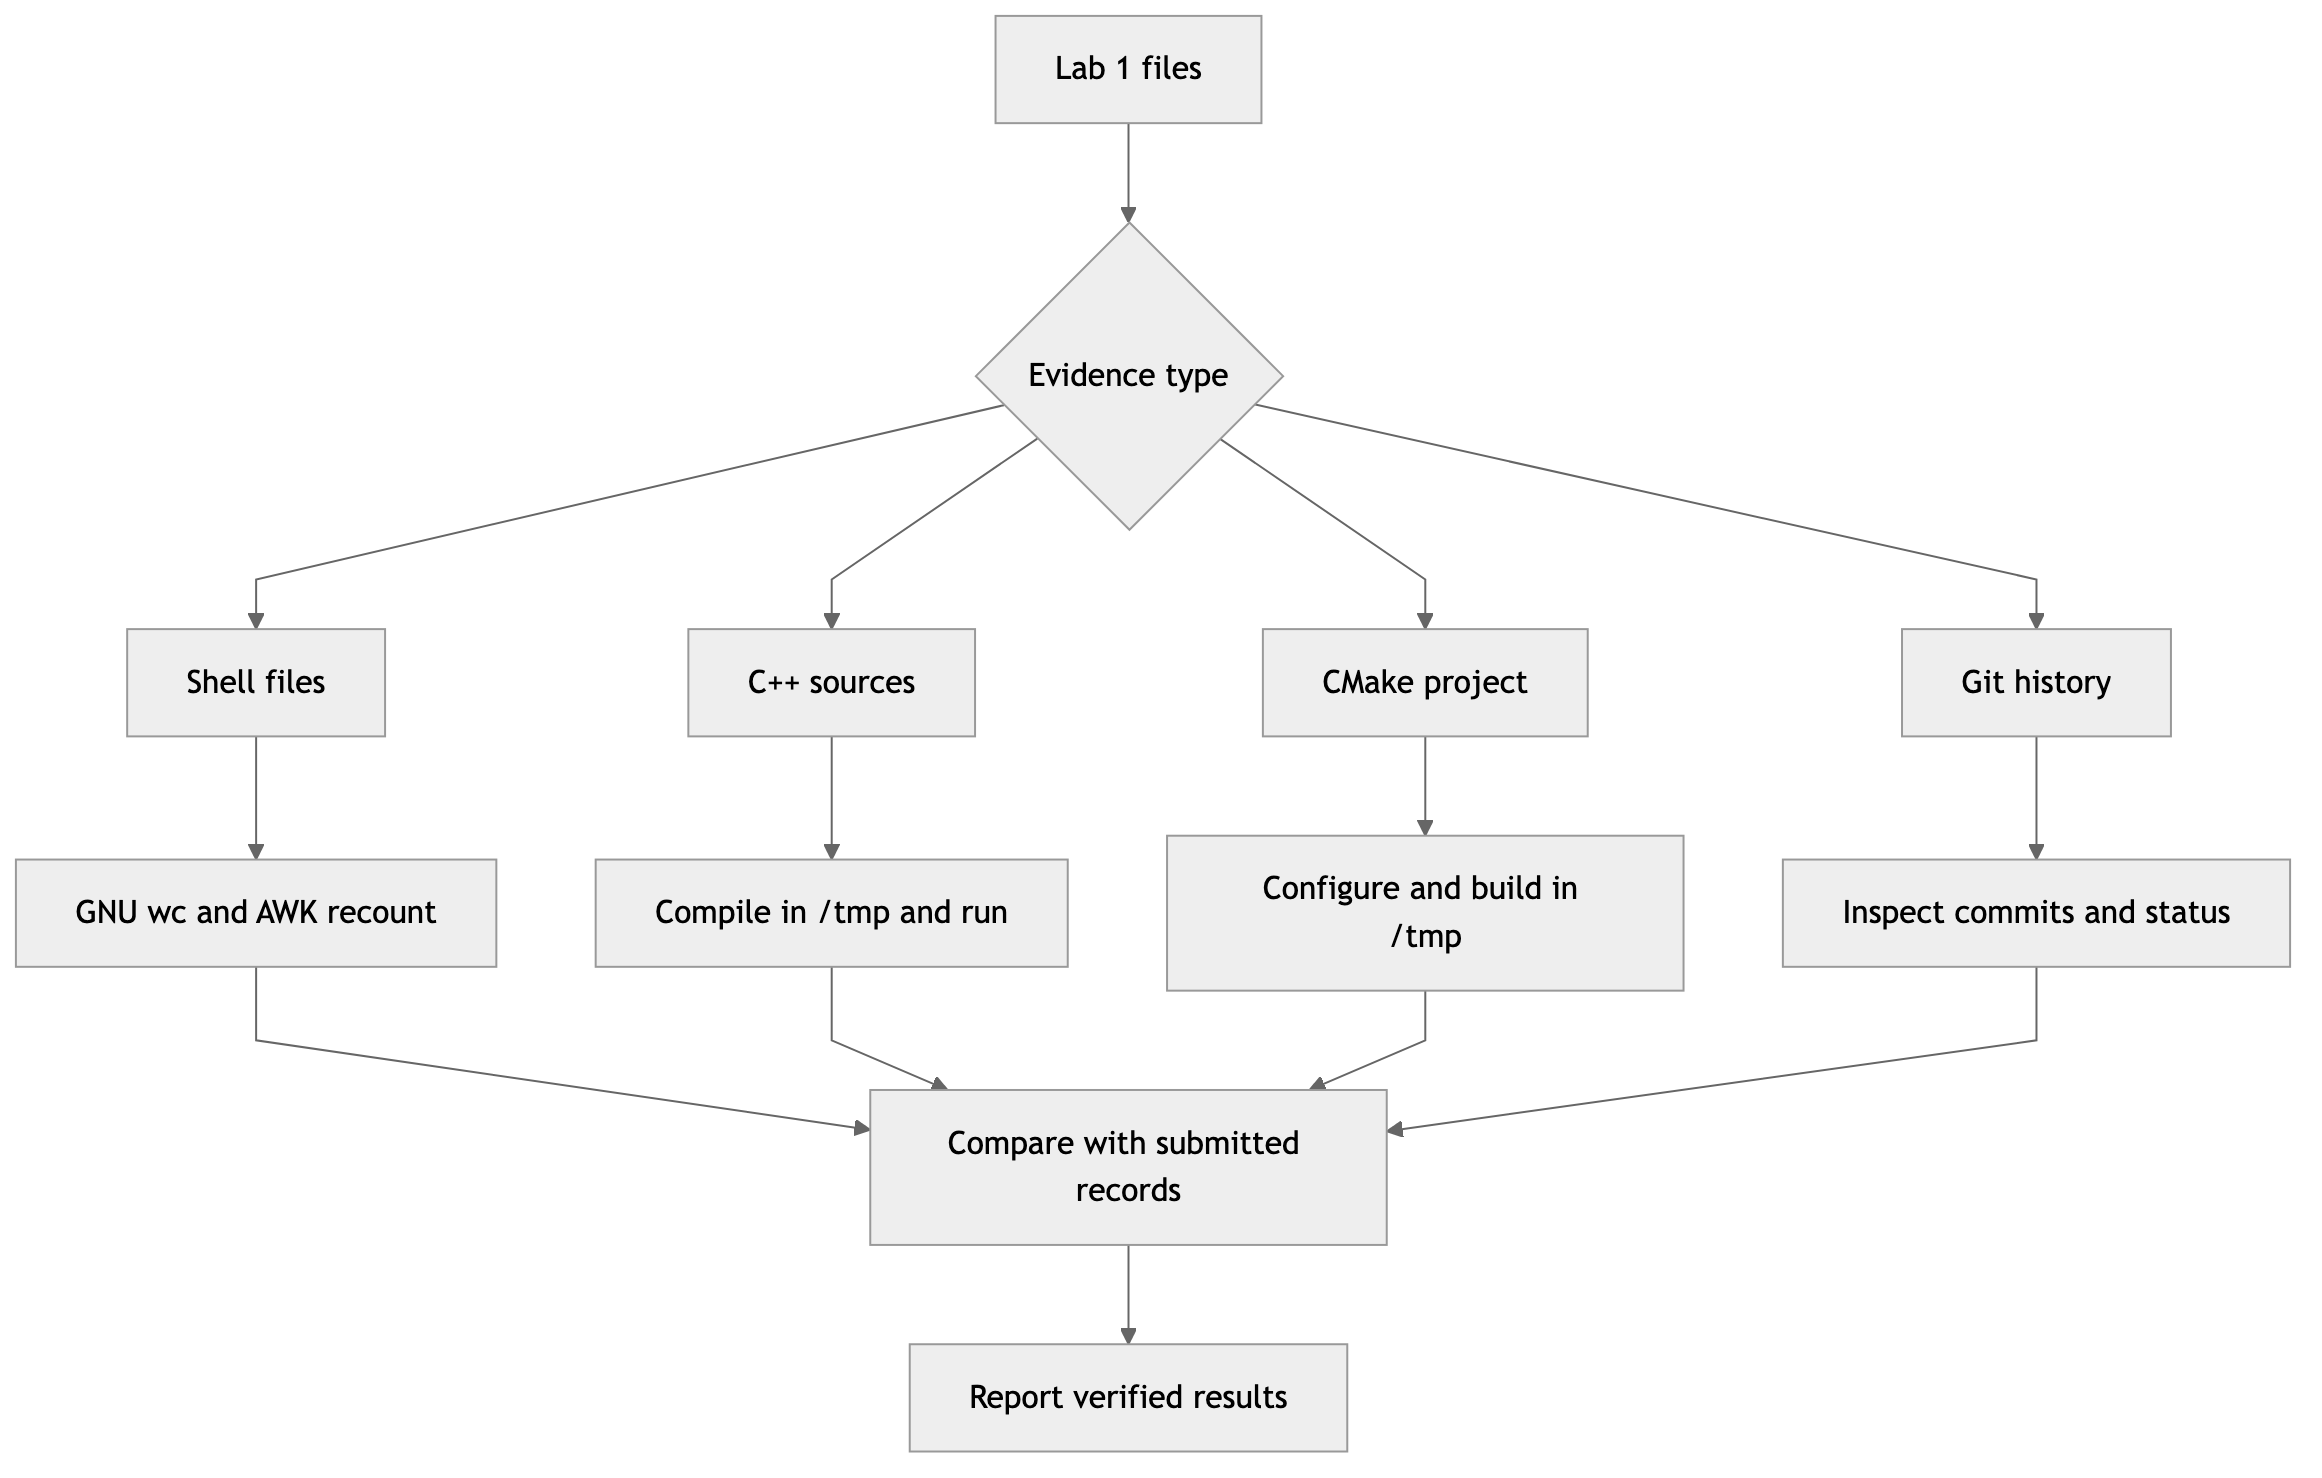
\includegraphics[width=0.96\columnwidth]{figures/verification_workflow.png}
  \caption{Lab 1 verification procedure. Build artifacts were written to temporary directories.}
  \label{fig:verification}
\end{figure}

\subsection{Shell Verification}

The following commands were used to count the contents of \texttt{dante.txt}:

\begin{lstlisting}[language=bash]
wc -l -w dante.txt
awk 'NF {n++} END {print n}' dante.txt
\end{lstlisting}

\texttt{wc -l} counts newline-terminated lines, while \texttt{wc -w} counts words according to the tool and locale rules. The AWK condition \texttt{NF} selects only lines containing at least one field, so blank lines do not increase \texttt{n}. The three outputs therefore give the total line count, word count, and nonblank line count.

\texttt{fortunes.txt} contains five separate \texttt{fortune} outputs, as required. Their presence also confirms that append redirection was used instead of overwriting earlier entries.

\subsection{C++ Implementation and Statistics}

\texttt{RandomVector} stores its data in a private \texttt{std::vector<double>}. The constructor first clamps a negative length or upper bound to zero, then generates $n$ values in $[0,\,m]$ using \texttt{rand()/RAND\_MAX}. The \texttt{print()} method writes the elements separated by spaces. For a vector $x_1,\ldots,x_n$, the mean is
\begin{equation}
  \bar{x}=\frac{1}{n}\sum_{i=1}^{n}x_i.
\end{equation}
All three statistical functions return 0 for an empty vector. For a nonempty vector, the minimum and maximum are found by linear scans without using the prohibited \texttt{<algorithm>} functions. The histogram maps values into $b$ equal-width bins. For element $i$, the bin index is
\begin{equation}
  k_i=\min\!\left(b-1,\left\lfloor
  \frac{x_i-x_{\min}}{x_{\max}-x_{\min}}b
  \right\rfloor\right).
\end{equation}
The upper clamp places the maximum value in the final bin. If every element is equal, the denominator is zero, so the program places all elements directly in the final bin. A nonpositive bin count or an empty vector produces no histogram. Figure~\ref{fig:randomvector} summarizes these control branches.

\begin{figure}[t]
  \centering
  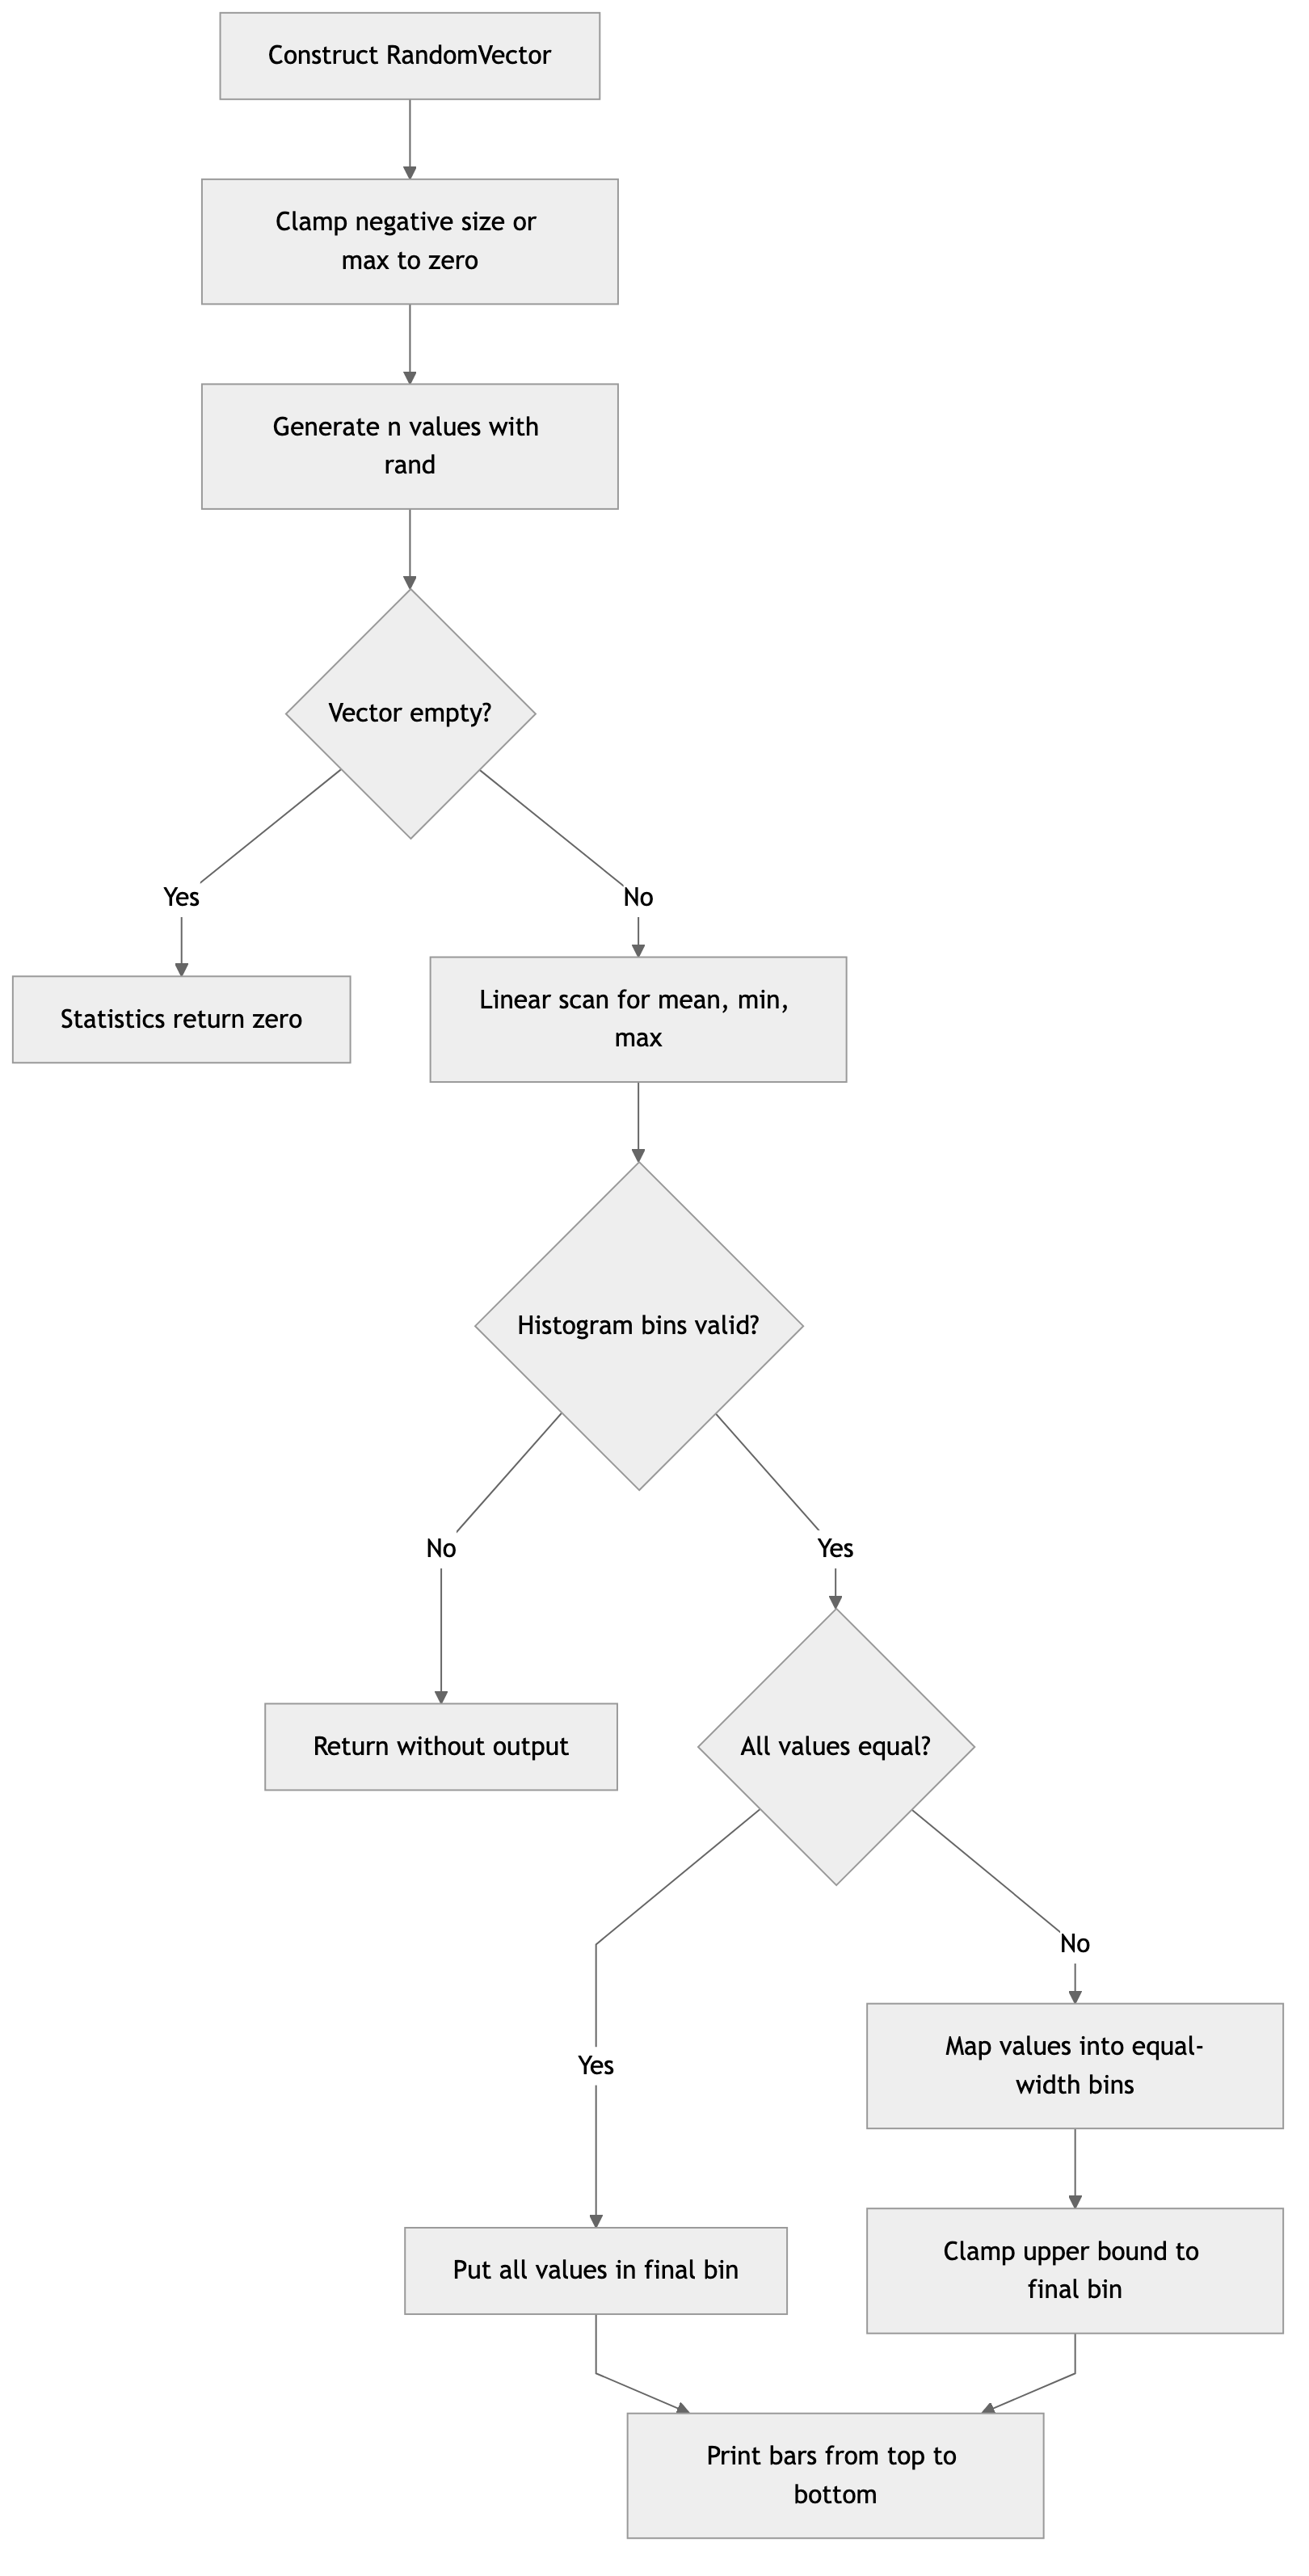
\includegraphics[width=0.96\columnwidth]{figures/random_vector_flow.png}
  \caption{RandomVector generation, statistics, and histogram output.}
  \label{fig:randomvector}
\end{figure}

The mean and extrema each require $O(n)$ time. Histogram counting takes $O(n)$ time and $O(b)$ additional space; the cost of printing also depends on the height of the largest bin. The test program uses the fixed seed 314159 so that its output is reproducible with the same C library implementation. The verification command was:

\begin{lstlisting}[language=bash]
g++ -std=c++11 -Wall -pedantic -o random_vector \
  main.cpp random_vector.cpp
./random_vector
\end{lstlisting}

\subsection{CMake Project}

In \texttt{lab1\_demo/CMakeLists.txt}, \texttt{add\_library} defines \texttt{mylib} from \texttt{my\_lib.cpp} and its header, and \texttt{add\_executable} defines \texttt{main}. The command \texttt{target\_link\_libraries(main PRIVATE mylib)} links the library to \texttt{main} without propagating the dependency to other targets. This matches the official example\cite{vnavcmake}.

The project was verified with separate source and build directories. The test host used CMake 3.28.3. Both \texttt{cmake -S} and \texttt{cmake --build} returned exit status 0. The resulting executable printed \texttt{Hello world!} and \texttt{In library}. These lines originate from the main program and the library function, respectively, and confirm that the link was successful. Figure~\ref{fig:cmake} distinguishes compilation of the library from compilation of the program that calls it. The build log records the static library before the executable, consistent with this dependency.

\begin{figure}[t]
\centering
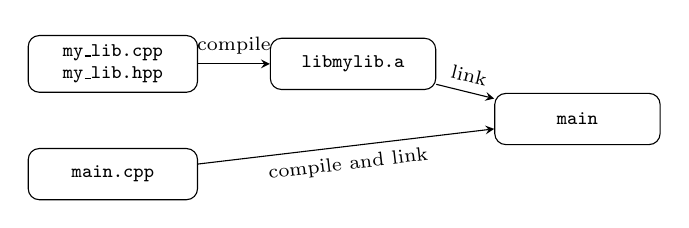
\begin{tikzpicture}[>=stealth, font=\scriptsize]
  \node[draw, rounded corners, align=center, minimum width=2.15cm, minimum height=0.65cm] (libsrc) at (0,1.2) {\texttt{my\_lib.cpp}\\\texttt{my\_lib.hpp}};
  \node[draw, rounded corners, align=center, minimum width=2.15cm, minimum height=0.65cm] (mainsrc) at (0,-0.2) {\texttt{main.cpp}};
  \node[draw, rounded corners, align=center, minimum width=2.1cm, minimum height=0.65cm] (lib) at (3.05,1.2) {\texttt{libmylib.a}};
  \node[draw, rounded corners, align=center, minimum width=2.1cm, minimum height=0.65cm] (main) at (5.9,0.5) {\texttt{main}};
  \draw[->] (libsrc) -- node[above]{compile} (lib);
  \draw[->] (lib) -- node[above, sloped]{link} (main);
  \draw[->] (mainsrc) -- node[below, sloped]{compile and link} (main);
\end{tikzpicture}
\caption{CMake target dependencies observed in the source configuration and build log.}
\label{fig:cmake}
\end{figure}

\section{Results}

\subsection{Deliverable Coverage}

Table~\ref{tab:coverage} lists the deliverables, evidence, and verification status in the order used by the official assignment. ``Verified'' means that the file contents match the corresponding requirement. ``Compiled'' and ``Built and executed'' also include evidence from actual execution.

\begin{table}[t]
\caption{Official requirements and repository evidence}
\label{tab:coverage}
\centering
\footnotesize
\begin{tabular}{p{0.18\columnwidth}p{0.49\columnwidth}p{0.18\columnwidth}}
\toprule
Item & Evidence & Result \\
\midrule
Git & Commit history; Lab 1 files in \texttt{15f3843} & Verified \\
Shell 1 & \texttt{dante.txt}, \texttt{exercise1.txt} & GNU counts match \\
Shell 2 & \texttt{fortunes.txt}, five outputs & Verified \\
C++ basics & Ten answers in \texttt{cpp\_exercises\_answers.md} & Verified \\
Random Vector & All six required interfaces & Compiled \\
CMake & Four required source files & Built and executed \\
\bottomrule
\end{tabular}
\end{table}

\subsection{Shell Results}

GNU \texttt{wc} reproduced the three values recorded in \texttt{exercise1.txt}, as shown in Table~\ref{tab:shell}. All three differences are zero, so the recorded values can be regenerated from the current input. The nonblank-line count is 14,338 out of 19,567 total lines; subtraction leaves 5,229 lines without fields under the AWK test. This is a derived count, not an additional shell measurement.

The same \texttt{dante.txt} file, with SHA-256 prefix and suffix \texttt{1cd578e1...c279}, produced 97,765 words on macOS and 97,676 words on GNU/Linux. The identical file hash rules out different input contents. Figure~\ref{fig:word-compare} isolates the 89-word difference, about 0.091\% of the GNU count. Its horizontal axis is truncated to make that small difference visible; the labels give the full counts.

\begin{figure}[t]
\centering
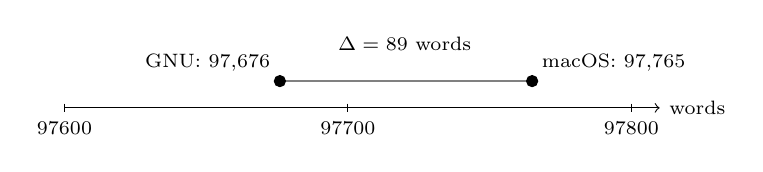
\begin{tikzpicture}[x=0.036cm,y=0.68cm,font=\scriptsize]
  \draw[->] (0,0) -- (210,0) node[right]{words};
  \foreach \x/\lab in {0/97600,100/97700,200/97800} {
    \draw (\x,0.08) -- (\x,-0.08) node[below]{\lab};
  }
  \draw[thick,gray] (76,0.5) -- (165,0.5);
  \filldraw[black] (76,0.5) circle (2pt) node[above left]{GNU: 97,676};
  \filldraw[black] (165,0.5) circle (2pt) node[above right]{macOS: 97,765};
  \node at (120,1.2) {$\Delta=89$ words};
\end{tikzpicture}
\caption{Word counts for the same input file. The horizontal axis starts at 97,600.}
\label{fig:word-compare}
\end{figure}

\begin{table}[t]
\caption{Recorded and verified GNU/Linux counts for \texttt{dante.txt}}
\label{tab:shell}
\centering
\footnotesize
\begin{tabular}{lrrr}
\toprule
Metric & Recorded & Verified & Difference \\
\midrule
Total lines & 19,567 & 19,567 & 0 \\
Words & 97,676 & 97,676 & 0 \\
Nonblank lines & 14,338 & 14,338 & 0 \\
\bottomrule
\end{tabular}
\end{table}

\subsection{RandomVector Results}

The program was compiled with GCC 13.3.0 on Ubuntu 24.04.5. The C++11 build enabled \texttt{-Wall -pedantic} and produced no compiler warnings. Compilation and execution both returned status 0. The program generated 20 values, with statistics shown in Table~\ref{tab:rv}. The mean lies between the minimum and maximum, and both the element count and histogram bin count match the arguments in the test program. Figure~\ref{fig:sequence} plots the 20 values in their printed order. The minimum is the sixth value and the maximum is the seventeenth; the dashed line marks the reported mean. The displayed values span 0.9547856, and ten lie above the reported mean while ten lie below it. These quantities were calculated from the 20 printed values.

\begin{figure}[!htbp]
\centering
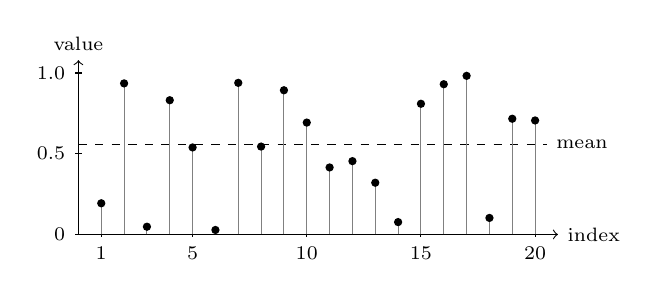
\begin{tikzpicture}[x=0.29cm,y=2.05cm,font=\scriptsize]
  \draw[->] (0,0) -- (21,0) node[right]{index};
  \draw[->] (0,0) -- (0,1.08) node[above]{value};
  \foreach \x in {1,5,10,15,20} \draw (\x,0.018) -- (\x,-0.018) node[below]{\x};
  \foreach \y/\lab in {0/0,0.5/0.5,1/1.0} \draw (0.15,\y) -- (-0.15,\y) node[left]{\lab};
  \draw[dashed] (0,0.55804) -- (20.5,0.55804) node[right]{mean};
  \foreach \x/\v in {1/0.193146,2/0.935807,3/0.0478698,4/0.831597,5/0.539111,6/0.0278694,7/0.93919,8/0.544454,9/0.893339,10/0.693182,11/0.415163,12/0.454242,13/0.320536,14/0.0766892,15/0.809584,16/0.93073,17/0.982655,18/0.102505,19/0.716924,20/0.706215} {
    \draw[gray] (\x,0) -- (\x,\v);
    \fill (\x,\v) circle (1.5pt);
  }
\end{tikzpicture}
\caption{The 20 printed RandomVector values in output order; the dashed line is the reported mean, 0.55804.}
\label{fig:sequence}
\end{figure}
\FloatBarrier

\begin{table}[t]
\caption{Verified results for \texttt{RandomVector(20)}}
\label{tab:rv}
\centering
\footnotesize
\begin{tabular}{lr}
\toprule
Metric & Result \\
\midrule
Elements & 20 \\
Random seed & 314159 \\
Mean & 0.55804 \\
Minimum & 0.0278694 \\
Maximum & 0.982655 \\
Histogram bins & 5 \\
\bottomrule
\end{tabular}
\end{table}

The corresponding text histogram is:

\noindent\begin{minipage}{0.95\columnwidth}
\begin{lstlisting}
                ***
                ***
***             ***
***     ***     ***
***     *** *** ***
***     *** *** ***
*** *** *** *** ***
\end{lstlisting}
\end{minipage}

The five bin counts reconstructed from that output are 5, 1, 4, 3, and 7. They sum to 20, matching the generated element count. The final bin contains 35\% of the sample, while the second bin contains one value (5\%). Figure~\ref{fig:histogram} displays these counts with a numeric vertical axis, which the terminal histogram does not provide. The bin width calculated from the displayed extrema is approximately 0.19096; the final interval includes the maximum.

\begin{figure}[t]
\centering
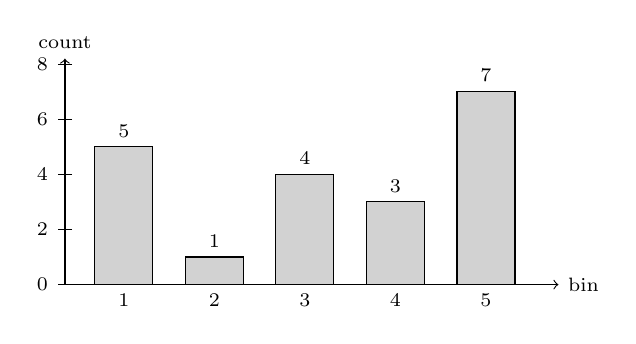
\begin{tikzpicture}[x=1.15cm,y=0.35cm,font=\scriptsize]
  \draw[->] (0.35,0) -- (5.8,0) node[right]{bin};
  \draw[->] (0.35,0) -- (0.35,8.2) node[above]{count};
  \foreach \y in {0,2,4,6,8} \draw (0.43,\y) -- (0.27,\y) node[left]{\y};
  \foreach \x/\c in {1/5,2/1,3/4,4/3,5/7} {
    \draw[fill=gray!35] (\x-0.32,0) rectangle (\x+0.32,\c);
    \node[above] at (\x,\c) {\c};
    \node[below] at (\x,0) {\x};
  }
\end{tikzpicture}
\caption{Five-bin frequency analysis reconstructed from the recorded RandomVector output ($n=20$).}
\label{fig:histogram}
\end{figure}

\noindent\begin{minipage}{\columnwidth}
\begin{lstlisting}[language=bash,basicstyle=\ttfamily\tiny]
$ grep '^PRETTY_NAME=' /etc/os-release
PRETTY_NAME="Ubuntu 24.04.5 LTS"
$ g++ --version | head -n 1
g++ (Ubuntu 13.3.0-6ubuntu2~24.04.1) 13.3.0
$ cmake --version | head -n 1
cmake version 3.28.3
$ wc -l -w dante.txt
 19567  97676 dante.txt
$ awk 'NF {n++} END {print n}' dante.txt
14338
$ /tmp/lab1-report-randomvector/random_vector
Mean: 0.55804
Min: 0.0278694
Max: 0.982655
$ cmake --build /tmp/lab1-report-cmake
[100%] Built target main
$ /tmp/lab1-report-cmake/main
Hello world!
In library
\end{lstlisting}
\end{minipage}

\section{Discussion}

\texttt{RandomVector} implements all six required interfaces. Its statistical functions use explicit loops, satisfying the restriction against obtaining extrema directly through \texttt{<algorithm>}. Boundary handling is located in the constructor, the statistical functions, and the entry to \texttt{printHistogram()}. Negative lengths, negative upper bounds, empty vectors, and nonpositive bin counts therefore have defined behavior. A separate branch for identical values prevents division by zero during histogram construction.

The histogram first counts the values in each bin and then prints rows from the highest level downward. The plotted counts and terminal output agree bin by bin. The chart also makes it possible to check that no generated value was lost during binning: $5+1+4+3+7=20$. The high count in the final bin describes this one 20-value sample; it is not evidence of a population-level distribution.

Platform differences appeared in both the shell counts and pseudorandom values. GNU and BSD toolchains returned different word counts for the same \texttt{dante.txt}, while glibc and macOS libc generated different \texttt{rand()} sequences from the same source and seed. Final numbers alone cannot explain these differences, so a complete verification record should also include the input hash, operating system, and tool versions.

\balance
\section{Limitations}

This report verifies the available files and newly generated output; it cannot reconstruct every action taken when the experiment was first completed. Compilation and execution show only that the current materials pass the reported checks. They do not cover untested environments, inputs, or boundary conditions. Version history shows that files were committed, but it cannot independently establish the state, access permissions, or ownership of a remote repository.

\section{Conclusion}

The required shell exercise, C++ warm-up answers, \texttt{RandomVector} implementation, and CMake files are present. The GNU shell counts on Ubuntu 24.04.5 match the submitted record, and both \texttt{RandomVector} and the CMake example compiled and executed successfully.

\begin{thebibliography}{4}
\bibitem{vnavlab1}
MIT SPARK Lab, ``VNAV 2023 Lab 1,'' 2023. [Online]. Available: \url{https://vnav.mit.edu/labs_2023/lab1/}

\bibitem{vnavexercises}
MIT SPARK Lab, ``VNAV 2023 Lab 1: Exercises,'' 2023. [Online]. Available: \url{https://vnav.mit.edu/labs_2023/lab1/exercises.html}

\bibitem{vnavcmake}
MIT SPARK Lab, ``VNAV 2023 Lab 1: Build with CMake,'' 2023. [Online]. Available: \url{https://vnav.mit.edu/labs_2023/lab1/cmake.html}

\bibitem{labbrief}
``Lab 1: Linux, C++, Git,'' course note. [Online]. Available: \url{https://spurious-cornflower-507.notion.site/Lab-1-Linux-C-Git-e788685e06a84200ae587ffe64258c76}
\end{thebibliography}

\end{document}
